%   % !TEX root = ../../VIII,3_Rahmen-TeX_9-0.tex
%  
%   Band VIII, 3 N.~?? 	
%   Signatur/Tex-Datei:	LH_37_05_159-160
%   RK-Nr. 	57271
%				
%   Überschrift: 	De vi ictus
%   Datierung:		11. (21.) Juni 1677 (eigh.)
%   edlabels:			11
%   Diagramme: 		2
%
%
%
\selectlanguage{ngerman}
\frenchspacing
%
\begin{ledgroupsized}[r]{120mm}
\footnotesize
\pstart
\noindent\textbf{Überlieferung:}
\pend
\end{ledgroupsized}
%
\begin{ledgroupsized}[r]{114mm}
\footnotesize
\pstart \parindent -6mm
\makebox[6mm][l]{\textit{L}}%
Konzept:
LH~XXXVII~5, Bl.~159\textendash160. 
Ein Bogen~4\textsuperscript{o}; Wasserzeichen im Falz; Ränder beschnitten; Papiererhaltungsmaßnahmen.
Vier Seiten.
\pend
\end{ledgroupsized}
%
\begin{ledgroupsized}[r]{114mm}
\footnotesize
\pstart
\parindent -6mm
\makebox[6mm][l]{\textit{E}}%
(tlw.) \textsc{Fichant} 1994, S.~384\textendash387\cite{01056}. 
\pend%
\end{ledgroupsized}
%
%
\selectlanguage{latin}
\frenchspacing
% \newpage%
\vspace{8mm}
\pstart%
\normalsize%
\noindent%
\lbrack159~r\textsuperscript{o}\rbrack\
\pend 
%
%
\pstart
\raggedleft 11 Jun.\ 1677
\pend 
\count\Bfootins=1100%
\count\Afootins=1100%
\count\Cfootins=1100
%
\pstart
\centering
De vi ictus\protect\index{Sachverzeichnis}{vis ictus}. 
\pend 
\vspace{0.5em}
\pstart\noindent
Danda opera est, ut tandem aliquando vim ictus\protect\index{Sachverzeichnis}{vis ictus} explicemus,
vis ictus\protect\index{Sachverzeichnis}{vis ictus} intelligi potest ex dolore%
\protect\index{Sachverzeichnis}{dolor} sentientis, ex corporis icti ruptura,%
\protect\index{Sachverzeichnis}{ruptura corporis icti}
itemque ex repercussu,%
\protect\index{Sachverzeichnis}{repercussus} si icta sint Elastica. Ante omnia
autem
%
\edtext{patet vim}{\lemma{patet}\Bfootnote{\textit{(1)}~ictum non posse \textit{(2)}~vim~\textit{L}}}
%%%
ictum%
\protect\index{Sachverzeichnis}{vis ictus} non posse esse
majorem quam potentiam\protect\index{Sachverzeichnis}{potentia}%
\protect\index{Sachverzeichnis}{potentia amborum corporum concurrentium} seu vim%
\protect\index{Sachverzeichnis}{vis}\protect\index{Sachverzeichnis}{vis amborum corporum concurrentium} amborum corporum concurrentium.
Patet etiam potentiam\protect\index{Sachverzeichnis}{potentia} debere manere eandem in
%
\edlabel{37_05_159-160_2a}%
\edtext{}{% NEUER ABSATZ UND VARIANTEN – "summa. Si"
{\xxref%
{37_05_159-160_2a}{37_05_159-160_2b}}%
\lemma{summa.}%
\Bfootnote{%
\textit{(1)}~Si corpus incurrat in aliud corpus quiescens, tunc ictu\protect\index{Sachverzeichnis}{ictus} ipso infligit ei \textit{(2)}~Si \textit{L}\
}}%
summa.
\pend
%
\pstart
Si%
\edlabel{37_05_159-160_2b}
%
corpus
%%
\edtext{incurrat in murum%
\protect\index{Sachverzeichnis}{murus} immobilem,}{\lemma{incurrat in}\Bfootnote{\textit{(1)}~aliud immobile, \textit{(2)}~murum \textit{(3)}~murum immobilem,~\textit{L}}}
%%
vis ictus\protect\index{Sachverzeichnis}{vis ictus}
tanta est, quanta est vis corporis incurrentis.%
\protect\index{Sachverzeichnis}{corpus incurrens}
%
\pend \pstart 
%
Eadem erit vis ictus\protect\index{Sachverzeichnis}{vis ictus} sive ego incurram in murum,%
\protect\index{Sachverzeichnis}{murus} sive murus%
\protect\index{Sachverzeichnis}{murus}
incurrat in me, et in momento concursus%
\protect\index{Sachverzeichnis}{momentum concursus} fingatur factus immobilis
me semper mobili
%
\edlabel{37_05_159-160_3a}%
\edtext{}{% NEUER ABSATZ UND VARIANTEN – manente...
{\xxref%
{37_05_159-160_3a}{37_05_159-160_3b}}%
\lemma{}%
\Bfootnote{%
manente. \textbar\ Sed \lbrack...\rbrack\ accipere. \textit{erg.}\ \textbar\ \textit{(1)}~Unde \textit{(2)}~Si~\textit{L}}}%
manente. Sed tunc fingendum est causam immobilitatis muri reliquam vim accipere.
\pend
%
\vspace{1.5em} %%%%%%%%% Diagramm 1
\centerline{%
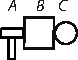
\includegraphics[width=0.15\textwidth]{%
gesamttex/edit_VIII,3/images/LH_37_05_159-160_d1_159r.pdf%
}} 
\vspace{0.5em}
\centerline{%
\lbrack\textit{Fig.~1}\rbrack%
}
% \newpage%
\vspace{1.2em}
%
\pstart
Si%
\edlabel{37_05_159-160_3b}
%
%%
malleo\protect\index{Sachverzeichnis}{malleus} \textit{A} percutiam
corpus immobile \textit{C}
%%
\edtext{egoque vi}{\lemma{egoque}\Bfootnote{\textit{(1)}~malleum\protect\index{Sachverzeichnis}{malleus} \textit{(2)}~vi~\textit{L}}}
%%
brachiorum impediam mallei\protect\index{Sachverzeichnis}{malleus} repercussionem\protect\index{Sachverzeichnis}{repercussio},
tunc corpus \textit{C} vi ictus\protect\index{Sachverzeichnis}{vis ictus} tanta propelletur, quanta est mallei\protect\index{Sachverzeichnis}{malleus}.
Longe major est vis ictus\protect\index{Sachverzeichnis}{vis ictus} si murus incurrat in me immobilem
eadem celeritate qua
%%
\edtext{ego incurrerem}{\lemma{ego}\Bfootnote{\textit{(1)}~incurro \textit{(2)}~incurreram \textit{(3)}~incurrerem~\textit{L}}} 
%%
in murum%
\protect\index{Sachverzeichnis}{murus} 
%%
%
\edlabel{37_05_159-160_4a}%
\edtext{}{% NEUER ABSATZ UND VARIANTEN – "immobile. Quaeritur"
{\xxref%
{37_05_159-160_4a}{37_05_159-160_4b}}%
\lemma{immobilem.}%
\Bfootnote{%
\textit{(1)}~Si \textit{(a)}~ego incurram in \textit{(aa)}~corp \textit{(bb)}~corpus mobile, aut si co \textit{(b)}~\textbar\ mo \textit{streicht Hrsg.}\ \textbar\  \textit{(2)}~Quaeritur \textit{L}\
}}%
immobilem.
\pend
%
\pstart
\hspace{1mm}\hspace{-1mm}% Trick, weil \edlabel nicht zu \par-Beginn sein darf
\edlabel{37_05_159-160_9a}%		Referenzierung
Quaeritur%
\edlabel{37_05_159-160_4b}
%
an idem sit ictus,\protect\index{Sachverzeichnis}{ictus} duorum corporum mobilium
quiescentium,%
\protect\index{Sachverzeichnis}{corpus quiescens}
%%
\edtext{licet}{\lemma{}\Bfootnote{licet \textit{erg.}~\textit{L}}}
%%
in utrovis ponatur motus.
\pend 
%
\pstart
%%
\edtext{%
\edtext{Ostendi in alia scheda 11 Jun.\ 1677}{\lemma{Ostendi}\Bfootnote{\textit{(1)}~supra \textit{(2)}~in alia scheda 11 Jun.\ 1677~\textit{L}}}
%%
etsi corpora ex eadem distantia\protect\index{Sachverzeichnis}{distantia} concurrerint, non
tamen ideo eundem semper ictum\protect\index{Sachverzeichnis}{ictus} posse inferre.% Referenzierung
\edlabel{37_05_159-160_9b}}{%
\lemma{Ostendi \lbrack...\rbrack\ inferre}%
\Cfootnote{%
Siehe die Passage auf S.~\refpassage{37_05_157-158_3a}{37_05_157-158_3b} von N.~\ref{57270}, das Leibniz allerdings auf den 10.\ (20.) Juni 1677 datiert hat.}}
%
%
\pend
%
\pstart
Si corpus incurrat in aliud quiescens se
%%
minus,%
\protect\index{Sachverzeichnis}{incursus corporis in quiescens minus} utique
%%
continuabit
motum, si jam %
corpus quiescens\protect\index{Sachverzeichnis}{corpus quiescens} una cum ipso procederet
minueretur celeritas in ea ratione, in qua massa\protect\index{Sachverzeichnis}{massa} corporum praecedentium
aucta esset. Ergo et %
corpus incurrens\protect\index{Sachverzeichnis}{corpus incurrens} de sua
potentia\protect\index{Sachverzeichnis}{potentia} nonnihil amisit, in quantum scilicet alteri communicavit.
%
Nempe \lbrack159~v\textsuperscript{o}\rbrack\ ponamus corporis
%%
\edtext{incurrentis \textit{B} celeritatem esse \textit{f}.}{\lemma{incurrentis}\Bfootnote{\textit{(1)}~\textit{b} \textit{B} potentiam \textbar\ esse \textit{streicht Hrsg.}\ \textbar\ %
 \textit{(2)}~\textit{B} celeritatem esse \textit{f}.~\textit{L}}}
%%
Erit potentia\protect\index{Sachverzeichnis}{potentia}
ejus \textit{fb}, quae divisa per $a+b$ dabit celeritatem summae%
\protect\index{Sachverzeichnis}{summa corporum} 
%%
\edtext{corporum. Si nullo}{\lemma{corporum.}\Bfootnote{\textit{(1)}~Si amba \textit{(2)}~Si nullo~\textit{L}}}
%%
ictu\protect\index{Sachverzeichnis}{ictus} existente, neque perdita motus parte progredi intelligantur,
%%
\edtext{ergo celeritas}{\lemma{ergo}\Bfootnote{\textit{(1)}~potentia\protect\index{Sachverzeichnis}{potentia} corporum \textit{(2)}~celeritas~\textit{L}}}
%%
corporum progredientium esset 
%%
\rule[0cm]{0mm}{16pt}\edtext{$\displaystyle\frac{b}{a+b}\,f$, et potentia\protect\index{Sachverzeichnis}{potentia} quam}{\lemma{$\displaystyle\frac{b}{a+b}\,f$,}\Bfootnote{\textit{(1)}~et celeritas \textit{(2)}~et potentia\protect\index{Sachverzeichnis}{potentia} \textit{(a)}~corporis \textit{(b)}~quam~\textit{L}}}
%%
corpus%
\protect\index{Sachverzeichnis}{corpus quiescens}
%%
\edtext{quiescens accepisset}{\lemma{quiescens}\Bfootnote{\textit{(1)}~accepit \textit{(2)}~accepisset~\textit{L}}}
%%
foret
%%
\edtext{$\displaystyle\frac{ab}{a+b}\,f$, et}{\lemma{$\displaystyle\frac{ab}{a+b}\,f$, }\Bfootnote{\textit{(1)}~ quae si \textit{(2)}~et~\textit{L}}}
%%
tantundem quoque perdidisset corpus incurrens.%
\protect\index{Sachverzeichnis}{corpus incurrens} Ergo
vis ictus\protect\index{Sachverzeichnis}{vis ictus} foret
%%
%
\edlabel{37_05_159-160_5a}%
\edtext{}{% NEUER ABSATZ UND VARIANTEN – "Hac vi ictus"
{\xxref%
{37_05_159-160_5a}{37_05_159-160_5b}}%
\lemma{$\displaystyle\frac{ab}{a+b}\,f$.}%
\Bfootnote{%
\textit{(1)}~Ea vis corporibus \textit{A}, et \textit{B} in \textbar\ reciproca \textit{streicht Hrsg.}\ \textbar\ %
 magnitudinum ratione \textit{(a)}~distribuitur \textit{(b)}~distribuatur, \textit{(aa)}~sed in \textit{(bb)}~in quantum datur \textbar\ corpori \textit{A}, \textit{streicht Hrsg.}\ \textbar\ %
\textit{(2)}~Hac \textit{L}\
}}%
$\displaystyle\frac{ab}{a+b}\,f$.
\pend
%
\pstart
Hac%
\edlabel{37_05_159-160_5b}
%
%%
vi ictus%
\protect\index{Sachverzeichnis}{vis ictus} corpora se
%%
\rule[0cm]{0mm}{10pt}\edtext{subingrediuntur. Cum}{\lemma{subingrediuntur}\Bfootnote{\textit{(1)}~, interea \textit{(2)}~. Cum~\textit{L}}}
%%
enim corpus \textit{B}
corpori \textit{A} hanc potentiam\protect\index{Sachverzeichnis}{potentia} inferre conetur, 
%%
\edtext{flectitur utrumque}{\lemma{flectitur}\Bfootnote{\textit{(1)}~id antequam eam recipiat \textit{(2)}~utrumque~\textit{L}}}
%%
potius quam eam recipiat, quia scilicet flecti potest, 
%
(modo ictus tam sit fortis ut vincat connexionem\protect\index{Sachverzeichnis}{connexio corporis} corporis,) et tamdiu flectetur
%%
\edtext{donec vis}{\lemma{donec}\Bfootnote{\textbar\ residua \textit{gestr.}\ \textbar\ vis~\textit{L}}}
%%
connexionis\protect\index{Sachverzeichnis}{vis connexionis}
%%
\edtext{(quae semper augetur compressione\protect\index{Sachverzeichnis}{compressio})}{\lemma{}\Bfootnote{(quae semper augetur compressione) \textit{erg.}~\textit{L}}}
%%
major fiat residua vi flexionis.%
\protect\index{Sachverzeichnis}{vis flexionis}
%
Quo facto corpora compressa se repellent,
%%
\edtext{et ita}{\lemma{et}\Bfootnote{\textit{(1)}~vis qu \textit{(2)}~corpus \textit{(3)}~\textbar\ vis \textit{streicht Hrsg.}\ \textbar\ distribue \textit{(4)}~ita~\textit{L}}}
%%
corpus excipiens\protect\index{Sachverzeichnis}{corpus excipiens} propelletur dimidia potentia ictus,\protect\index{Sachverzeichnis}{potentia ictus}
%%
\edtext{corpus incurrens\protect\index{Sachverzeichnis}{corpus incurrens}}{\lemma{corpus}\Bfootnote{\textit{(1)}~excipiens \textit{(2)}~incurrens~\textit{L}}}
%%
repelletur altera dimidia, 
%%
\edtext{cumque idem progrediatur}{\lemma{cumque}\Bfootnote{\textit{(1)}~ita \textit{(2)}~idem \textit{(a)}~etiam accesserit \textit{(b)}~progrediatur~\textit{L}}}
%%
sua potentia\protect\index{Sachverzeichnis}{potentia} residua. Hinc
sive vincat, sive vincatur,
%%
\edtext{tunc progredietur}{\lemma{tunc}\Bfootnote{\textit{(1)}~vis \textit{(2)}~progredietur~\textit{L}}}
%%
aut regredietur
excessu\protect\index{Sachverzeichnis}{excessus potentiarum} harum pugnantium potentiarum, consumta autem sive 
destructa potentia\protect\index{Sachverzeichnis}{potentia destructa} in alterum corpus transferetur.
%
\pend 
%
\pstart
(\protect\vphantom)Hanc translationem\protect\index{Sachverzeichnis}{translatio} destructae potentiae\protect\index{Sachverzeichnis}{potentia destructa} in oppositum ita explico,
%
si ego pilam\protect\index{Sachverzeichnis}{pila} excipiam quietus reflectetur sua potentia\protect\index{Sachverzeichnis}{potentia},
%
si praeterea repercutiam, et manum in loco ictus\protect\index{Sachverzeichnis}{ictus} sistam, excipiet
omnem potentiam\protect\index{Sachverzeichnis}{potentia} quam non sentit manus.\protect\vphantom() 
%
\pend
%
\pstart
Dicere enim vim destructam%
\protect\index{Sachverzeichnis}{vis destructa} ipsi corpori dari, in quo destructa est\lbrack,\rbrack\ parum consentaneum videtur, si
%%
\edtext{potentia\protect\index{Sachverzeichnis}{potentia} alioqui}{\lemma{potentia\protect\index{Sachverzeichnis}{potentia}}\Bfootnote{\textit{(1)}~destructa tota transfertur in corpus \textit{(2)}~alioqui~\textit{L}}}
%%
destruenda tota in corpore altero recipitur, corpore uno existente irrepercutibili multo
magis si non quiescat tantum sed et plus quam quiescat, seu
in contrariam partem eat.
%
\pend \pstart
%
\lbrack160~r\textsuperscript{o}\rbrack\ Certum est et experimentis\protect\index{Sachverzeichnis}{experimentum} confirmatum, 
%
corpus incurrens in aequale quiescens
\protect\index{Sachverzeichnis}{incursus corporis in aequale quiescens} in ejus locum succedere,
%
et alterum 
%
\edlabel{37_05_159-160_6a}%
\edtext{}{% NEUER ABSATZ UND VARIANTEN – "impellere. Ita"
{\xxref%
{37_05_159-160_6a}{37_05_159-160_6b}}%
\lemma{impellere}%
\Bfootnote{%
\textit{(1)}~Jam \textit{(2)}~Ita~\textit{L}}}%
impellere.
\pend
%
\pstart
Ita%
\edlabel{37_05_159-160_6b}
%
observantur omnes regulae, scilicet tum potentiae\protect\index{Sachverzeichnis}{regula potentiae} tum 
compositionis\protect\index{Sachverzeichnis}{regula compositionis}.
\pend \pstart
%
\hspace{1mm}\hspace{-1mm}% Trick, weil \edlabel nicht zu \par-Beginn sein darf
%
\edlabel{37_05_159-160_11a}%
\edtext{}{% C-Footnote
{\xxref%
{37_05_159-160_11a}{37_05_159-160_11b}}%
\lemma{Jam \lbrack...\rbrack\ \lbrack fortioris\rbrack}%
\Cfootnote{%
Da in diesem Absatz die Körper \textit{a} und \textit{b} (bzw.\ \textit{A}) durchgehend als gleich, aber mit ungleichen Geschwindigkeiten bewegt, angenommen werden, ist die überlieferte Lesart \glqq potentiae minoris opponatur aequalis potentia majoris\grqq\ entweder mit der Prämisse nicht vereinbar oder in sich widersprüchlich.
%
Der Text wird entsprechend der Annahme geändert, dass Leibniz sich elliptisch ausgedrückt hat und mit \textit{potentia minoris} und \textit{majoris} eigentlich die Bewegungsgröße des langsameren bzw.\ schnelleren Körpers, die bei gleicher Masse eine jeweils kleinere bzw.\ größere \textit{potentia} besitzen, meint.
%
In der Parallelstelle auf S.~\refpassage{37_05_159-160_12a}{37_05_159-160_12b} hat Leibniz den Ausdruck \glqq majoris\grqq\ mit dem Wort \glqq fortioris\grqq\ kommentiert.}}%
%
Jam occurrant sibi duo corpora\protect\index{Sachverzeichnis}{corpora aequalia} 
%
\edtext{aequalia, tunc}{\lemma{aequalia,}\Bfootnote{\textit{(1)}~ponamus id quod minus \textbar\ est \textit{streicht Hrsg.}~\textbar\ %
 \textit{(2)}~tunc~\textit{L}}}
potentiae\protect\index{Sachverzeichnis}{potentia} 
%
\edtext{\lbrack debilioris\rbrack}{%
\lemma{}%
\Bfootnote{%
minoris %
\textit{L ändert Hrsg.}%
}}
%
opponatur aequalis
%
\edtext{potentia\protect\index{Sachverzeichnis}{potentia} \lbrack fortioris\rbrack.\edlabel{37_05_159-160_11b} Sit}{%
\lemma{potentia}%
\Bfootnote{%
\textbar\ majoris \textit{ändert Hrsg.} \textbar\ %
\textit{(1)}~\textbar\ Sit \textit{streicht Hrsg.}\ \textbar\ %
\textit{(a)}~\textit{ae}. \textit{bf}. %
\textit{(b)}~\textit{af} et $bf\, \sqcap$ %
\textit{(2)}~Sit%
~\textit{L}%
}}
%
\textit{ae}, \textit{Af}, et $f\,\sqcap\,e+g$, erit:
residua
%%
\edtext{ipsius corporis \textit{b}}{\lemma{ipsius}\Bfootnote{\textit{(1)}~\textit{a} \textit{(2)}~\textit{A} pot \textit{(3)}~corporis \textit{(a)}~\textit{a} \textit{(b)}~\textit{b}~\textit{L}}}
%%
(sive \textit{A}) potentia\protect\index{Sachverzeichnis}{potentia} \textit{Ag}.
%
Quod
%
\edtext{\lbrack si\rbrack}{%
\lemma{}%
\Bfootnote{%
si %
\textit{erg.\ Hrsg.}%
}}
%%
id incurrisset
%%
hac celeritate in corpus aequale quiescens%
\protect\index{Sachverzeichnis}{incursus corporis in aequale quiescens} \textit{a},
quievisset in ejus loco, eique dedisset celeritatem \textit{g}\lbrack;\rbrack\ in quantum 
autem ambo feruntur potentia\protect\index{Sachverzeichnis}{potentia} \textit{e}, eatenus ambo eadem potentia\protect\index{Sachverzeichnis}{potentia} 
reflectentur, ergo
%%
\edtext{patet corpus}{\lemma{patet}\Bfootnote{\textit{(1)}~alter \textit{(2)}~corpus~\textit{L}}}
%%
\textit{a} accipere $e+g$, et corpus \textit{b}
seu \textit{A} accipere solum \textit{e}, id est alternari 
%
\edlabel{37_05_159-160_1a}%	%B-Fn mit Absatz "celeritates"
\edtext{}{{\xxref{37_05_159-160_1a}{37_05_159-160_1b}}\lemma{}\Bfootnote{celeritates. 
\textit{(1)}~Videamus quid contingat, si ad ictum corporum explicandum fingamus ea concurrere aequali celeritate. \textit{(2)}~Si \textit{L}}}%
celeritates.
\pend
\newpage
%
%
%\vspace{2.0em} %%%%%%%%% Diagramm 2
\centerline{%
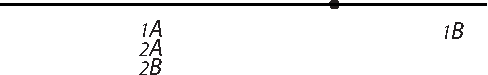
\includegraphics[width=0.6\textwidth]{%
gesamttex/edit_VIII,3/images/LH_37_05_159-160_d2_160r.pdf%
}} 
\vspace{0.5em}
\centerline{%
\lbrack\textit{Fig.~2}\rbrack%
}
% \newpage%
\vspace{1.5em}
%
\pstart
\edtext{}{%	Trick für FN-Diagramm
\lemma{\hspace*{1,6mm}%
\lbrack\textit{Fig.~2}\rbrack%
}\killnumber%
\Cfootnote{%
Ein gestrichener Entwurf zum Diagramm wird nicht wiedergegeben.%
}}%
Si\edlabel{37_05_159-160_1b} corpus unum incurrat in aliud quiescens,%
\protect\index{Sachverzeichnis}{incursus corporis in aliud quiescens} certum est ictum\protect\index{Sachverzeichnis}{ictus} aliquem
%%
\edtext{infligi. Si}{\lemma{infligi}\Bfootnote{\textit{(1)}~, et ictum illum eundem esse, qui f \textit{(2)}~. \textbar\ Addo \textit{streicht Hrsg.}\ \textbar\ %
ictum\protect\index{Sachverzeichnis}{ictus} illum eundem esse qui foret \textit{(3)}~. Si~\textit{L}}}
%%
corpora
%%
\edtext{duo occurrant}{\lemma{duo}\Bfootnote{\textit{(1)}~concurrant \textit{(2)}~occurrant~\textit{L}}}
%%
potentiis aequalibus, 
%%
\edtext{erit vis ictus\protect\index{Sachverzeichnis}{vis ictus} eadem cum potentia\protect\index{Sachverzeichnis}{potentia}}{\lemma{erit}\Bfootnote{%
\textit{(1)}~ictus idem %
\textit{(2)}~vis ictus eadem cum %
\textit{(a)}~potentiis %
\textit{(b)}~potentia~\textit{L}%
}}
%
utraque.
%
Si corpora duo occurrant potentiis inaequalibus,%
\protect\index{Sachverzeichnis}{potentiae inaequales} tunc vis ictus\protect\index{Sachverzeichnis}{vis ictus}
erit duplex\lbrack,\rbrack\ una quae est partis in majori, quae minori occurrenti aequalis est,
altera quae
%
\edtext{fit a residua
%
\edlabel{37_05_159-160_12a}%
\edtext{}{% 
{\xxref%
{37_05_159-160_12a}{37_05_159-160_12b}}%
\lemma{}%
\Afootnote{%
\textit{Zwischen den Zeilen, oberhalb} majoris:\enspace fortioris}}%
%
majoris\edlabel{37_05_159-160_12b}}{\lemma{fit}\Bfootnote{\textit{(1)}~a majori \textit{(2)}~a residua \textit{(a)}~minoris \textit{(b)}~majoris ~\textit{L}}}
%%
parte in minus consideratum ut 
%%
\edtext{quiescens. Omnis}{\lemma{quiescens.}\Bfootnote{\textit{(1)}~De  \textit{(2)}~Si \textit{(3)}~Omnis~\textit{L}}}
%%
\edtext{potentia\protect\index{Sachverzeichnis}{potentia} quae in uno}{\lemma{potentia\protect\index{Sachverzeichnis}{potentia}}\Bfootnote{\textit{(1)}~destructa \textit{(2)}~in uno \textit{(3)}~quae~\textit{L}}}
%%
corpore destrueretur, transfertur
in aliud corpus, alioqui periret, scilicet per repercussionem\protect\index{Sachverzeichnis}{repercussio}.
\pend \pstart
Explicandum est ante omnia quid fiat corpore in quiescens incurrente,%
\protect\index{Sachverzeichnis}{incursus corporis in aliud quiescens} et quae
tunc sit  
%%
vis ictus.%
\protect\index{Sachverzeichnis}{vis ictus} Vis ictus%
\protect\index{Sachverzeichnis}{vis ictus} semper aequaliter inter
duo corpora distribuitur, ita tamen ut aliquo corpore non recipiente destructa pars potentiae\protect\index{Sachverzeichnis}{potentia}
in alterum transferatur.%
\pend
%
\pstart
Videtur illud pro certo sumi posse, si eadem
%%
\edtext{potentia\protect\index{Sachverzeichnis}{potentia} sit}{\lemma{potentia\protect\index{Sachverzeichnis}{potentia}}\Bfootnote{\textit{(1)}~sibi occurrat ex ead \textit{(2)}~ sit~\textit{L}}}
%%
quae agat ex eadem distantia,%
\protect\index{Sachverzeichnis}{distantia} eandem esse
vim ictus\protect\index{Sachverzeichnis}{vis ictus}. Videtur enim ictus\protect\index{Sachverzeichnis}{ictus} et per distantiam\protect\index{Sachverzeichnis}{distantia} corporum, et per agentium potentiam\protect\index{Sachverzeichnis}{potentia}
determinari. Unde videndum an
%%
\edtext{sequatur ictus\protect\index{Sachverzeichnis}{vis ictus}}{\lemma{sequatur}\Bfootnote{\textit{(1)}~distantia \textit{(2)}~ictus~\textit{L}}}
%%
vim esse in ratione composita ex ratione distantiarum%
\protect\index{Sachverzeichnis}{distantia} et potentiarum\protect\index{Sachverzeichnis}{potentia} sibi oppositarum, \lbrack160~v\textsuperscript{o}\rbrack\ item an ista possint conciliari  
%
\edtext{cum illis quae prius constituimus
de compositione
ex opposita actione\protect\index{Sachverzeichnis}{actio opposita} et quiete\protect\index{Sachverzeichnis}{quies}.}{%
\lemma{cum \lbrack...\rbrack\ quiete}%
\Cfootnote{%
Siehe die Passage auf S.~\refpassage{37_05_159-160_9a}{37_05_159-160_9b}.}}
\pend \pstart
Videtur et certum esse, quod in corpus idem quiescens%
\protect\index{Sachverzeichnis}{corpus quiescens} idem ictus\protect\index{Sachverzeichnis}{ictus} 
%%
\edtext{infligatur a parvo}{\lemma{infligatur a}\Bfootnote{\textit{(1)}~magno \textit{(2)}~parvo~\textit{L}}}
%%
celeriter moto,%
\protect\index{Sachverzeichnis}{corpus parvum celeriter motum} qui infligitur a magno tanto tardius moto.%
\protect\index{Sachverzeichnis}{corpus magnum tardius motum} 
\pend \pstart
Hinc posito quid corpus aequale efficiat incurrens in aliud sibi aequale 
quiescens,%
\protect\index{Sachverzeichnis}{incursus corporis in aequale quiescens} videtur demonstrari posse quid efficiat corpus majus sed tardius motum.%
\protect\index{Sachverzeichnis}{corpus magnum tardius motum}
Unde ex hac unica regula videtur demonstrari posse, quicquid fieri debet de corpore
quiescente.%
\protect\index{Sachverzeichnis}{corpus quiescens} Verum ea regula ideo suspecta est, quod
supra cum
ea vellemus uti
collegimus semper
%%
\edtext{potentiam\protect\index{Sachverzeichnis}{potentia} transferri}{\lemma{potentiam\protect\index{Sachverzeichnis}{potentia}}\Bfootnote{\textit{(1)}~alternari \textit{(2)}~alternis \textit{(3)}~transferri~\textit{L}}}
%%
de corpore in corpus, si
scilicet ea velimus uti generaliter. Hoc loco tamen
%%
\edlabel{37_05_159-160_7a}%
\edtext{}{% NEUER ABSATZ UND VARIANTEN – "videndum. Sit"
{\xxref%
{37_05_159-160_7a}{37_05_159-160_7b}}%
\lemma{videndum}%
\Bfootnote{%
\textit{(1)}~, quia non videtur id fieri \textit{(2)}~. Sit~\textit{L}}}%
videndum.
\pend
%
\pstart
\rule[0cm]{0mm}{20pt}Sit%
\edlabel{37_05_159-160_7b}
%%
$\begin{array}{c|c}
b.f. & a.e.\\
\hline
bm & ai
\end{array}$
sit $a\,\sqcap\,b$ et $e\,\sqcap\,0$. Erit $m\,\sqcap\,0$ et $i\,\sqcap\,f$ et $ai\,\sqcap\,bf$.%
\pend
%
\pstart\noindent
\rule[0cm]{0mm}{20pt}Jam sit
%%
\edtext{$\displaystyle\frac{\vspace{3pt} d.h \ | \ a.e}{d.n \ | \ a.v}$ manentibus}{\lemma{$\displaystyle\frac{\vspace{3pt} d.h \ | \ a.e}{d.n \ | \ a.v}$}\Bfootnote{\textit{(1)}~sitque rursus $e\,\sqcap\,0$. \textit{(2)}~pon \textit{(3)}~manentibus~\textit{L}}}
%%
$a.e.$ ut ante.
%
\pend \pstart\noindent
\rule[0cm]{0mm}{12pt}Posito jam $dh\,\sqcap\,bf$, ut eadem sit quae ante potentia incurrentis, debet
etiam eadem esse 
%%
\edtext{potentia\protect\index{Sachverzeichnis}{potentia} accepta}{\lemma{potentia\protect\index{Sachverzeichnis}{potentia}}\Bfootnote{\textit{(1)}~excepta ab \textit{(2)}~accepta~\textit{L}}}
%%
\rule[0cm]{0mm}{16pt}ab excipiente, seu fiet:
$av\,\sqcap\,ai$, ergo $v\,\sqcap\,i$. $h\,\sqcap\,\displaystyle\frac{bf}{d}\,\sqcap\,\displaystyle\frac{ai}{d}$.%
\pend
%
\pstart\noindent
\rule[0cm]{0mm}{10pt}Quaeritur \textit{n}. Scilicet $dn+av\,\sqcap\,
%%
\edtext{dh+ae$ ex}{\lemma{$dh+ae$.}\Bfootnote{\textit{(1)}~seu \textit{(2)}~ex~\textit{L}}}
%%
natura potentiae\protect\index{Sachverzeichnis}{potentia}
seu $dn+bf\,\sqcap\,dh$ quia 
%%
\edtext{$ae\,\sqcap\,0$. Est}{\lemma{$ae\,\sqcap\,0$.}\Bfootnote{\textit{(1)}~Ergo \textit{(2)}~ Est~\textit{L}}}
%%
autem $dh\,\sqcap\,bf$
ergo fit $dn+bf\,\sqcap\,bf$ seu fit 
%%
\edtext{$dn\,\sqcap\,0$, 
\edlabel{37_05_159-160_13a}ergo haec regula}{\lemma{$dn\,\sqcap\,0$}\Bfootnote{\textit{(1)}~. Ergo haec regula \textit{(2)}~, ergo haec regula~\textit{L}}}
%%
falsa est, ex qua sequeretur
%%
\edtext{semper permutari}{\lemma{semper}\Bfootnote{\textit{(1)}~alternari mut \textit{(2)}~permutari~\textit{L}}}
%%
potentias\protect\index{Sachverzeichnis}{potentia}.%
\edlabel{37_05_159-160_13b}
%
Unum quod responderi
%%
\edtext{potest argumento}{\lemma{potest}\Bfootnote{\textit{(1)}~, hoc est quod \textit{(2)}~argumento~\textit{L}}}
%%
est, quod corporis
ipsius magnitudo simul computari debet.
\pend 
\pstart
\hspace{1mm}\hspace{-1mm}% Trick, weil \edlabel nicht zu \par-Beginn sein darf
\edlabel{37_05_159-160_8a}%	%Zwecks Referenzierung im DCC
Si dicamus corpus semper totam suam potentiam\protect\index{Sachverzeichnis}{potentia} alteri dare, hoc ita intelligendum est, quod
dabit potius
%%
\edtext{Elaterio\protect\index{Sachverzeichnis}{elaterium} si}{\lemma{Elaterio}\Bfootnote{\textit{(1)}~seu s \textit{(2)}~ si~\textit{L}}}
%%
flexile est\lbrack,\rbrack\ porro tantum potentiae\protect\index{Sachverzeichnis}{potentia} impendi poterit in Elaterium\protect\index{Sachverzeichnis}{elaterium},
donec ejus resistentia\protect\index{Sachverzeichnis}{resistentia} fiat aequalis vi agentis, residuae potentiae\protect\index{Sachverzeichnis}{potentia} in opposita corpora
transferentur. Ictus autem tantus erit quanta est tota potentia\protect\index{Sachverzeichnis}{potentia tota}, sed non totus ictus\protect\index{Sachverzeichnis}{ictus}
operabitur ad repercussionem\protect\index{Sachverzeichnis}{repercussio}, nisi in quantum Elaterio\protect\index{Sachverzeichnis}{elaterium} non est fortior.%
\edlabel{37_05_159-160_8b}
\pend
\pstart
Non posse istas regulas semper observari de ictu\protect\index{Sachverzeichnis}{ictus}, vel ex eo patet, quod si corpus
aliquod motu suo aliud abripiat\lbrack,\rbrack\
%%
\edtext{non in}{\lemma{non}\Bfootnote{\textit{(1)}~id \textit{(2)}~in~\textit{L}}}
%%
id impingens, 
%
sed illud velut 
glutine\protect\index{Sachverzeichnis}{gluten} correptum, et secum transferens,
%
nihil plane aliud fiet, quam quod servata eadem
potentia\protect\index{Sachverzeichnis}{potentia} celeritas minuetur: Ut si currui\protect\index{Sachverzeichnis}{currus} currenti 
%%
\edtext{ego imponam aliquid.}{\lemma{ego}\Bfootnote{\textit{(1)}~injicam aliquid vel imponam \textit{(2)}~imponam aliquid.~\textit{L}}}
%%
\edlabel{37_05_159-160_10a}%
\edtext{}{% C-Footnote
{\xxref%
{37_05_159-160_10a}{37_05_159-160_10b}}%
\lemma{Opus \lbrack...\rbrack\ penduli}%
\Cfootnote{%
Einige der hier erwähnten Experimente werden im programmatischen Konzept \glqq Experiences à faire sur le mouvement\grqq\ von Ende September\textendash Oktober 1677 (N.~\ref{52278}) wieder aufgegriffen.}}%
%
Opus est experimentis\protect\index{Sachverzeichnis}{experimentum} ad hanc materiam de concursu determinandam. 
%
Quanta sit vis ictus\protect\index{Sachverzeichnis}{vis ictus} sciri poterit ex perdito motu, si
corpus incurrat\protect\index{Sachverzeichnis}{incursus corporis in aliud molle} in aliud 
%%
\edtext{molle\protect\index{Sachverzeichnis}{corpus molle} ita}{\lemma{molle}\Bfootnote{\textit{(1)}~cum quo postea pro \textit{(2)}~ita~\textit{L}}}
%%
ut postea simul procedant.
Hinc discemus quanta sit vis ictus.\protect\index{Sachverzeichnis}{vis ictus} Curabimus etiam inflatas pilas\protect\index{Sachverzeichnis}{pila inflata} in se
invicem incurrere, ut vim ictus\protect\index{Sachverzeichnis}{vis ictus} notemus\lbrack;\rbrack\ omnia ope penduli\protect\index{Sachverzeichnis}{pendulum}.%
\edlabel{37_05_159-160_10b}
\pend
\count\Bfootins=1200%
\count\Afootins=1200%
\count\Cfootins=1200
